\chapter{Experimentos}\label{cap_experimentos}

Como forma de avaliar o modelo proposto serão conduzidos dois principais experimentos.

\section{Detalhes da simulação}

A simulação foi feita em C++ utilizando o framework Auryn~\cite{zenkeLimits2014} e o código está disponível no repositório GitHub
do autor~\cite{cendronGithub2023}.

\section{Experimento 1: Formação de assembleias neuronais}

O primeiro experimento consiste em simular a RNP apresentando estímulos ao modelo de retina e analisar se a repetição dos
estímulos leva à formação de assembleias neuronais associadas a cada estímulo a longo prazo, com o objetivo de ter uma base de
comparação para o experimento 2, que terá o sono simulado. Os estímulos consistem em seis imagens simples de serem reconhecidas,
exibidas na Figura~\ref{fig_estimulos}, e são apresentados à rede de forma intercalada e aleatória. Quatro estímulos foram
reaproveitados do trabalho de~\citeonline{zenkeDiverse2015}, enquanto as figuras de diamante e de cruz foram adicionadas com o
intuito de colocar a RNP mais próxima do seu limite.

\begin{figure}[!ht]
\caption{Os seis estímulos apresentados à RNP durante os experimentos. As cores são apenas ilustrativas, como mencionado na Seção~\ref{subsection_retina}, os estímulos são binários.}
\centering{
\parbox{12cm}{
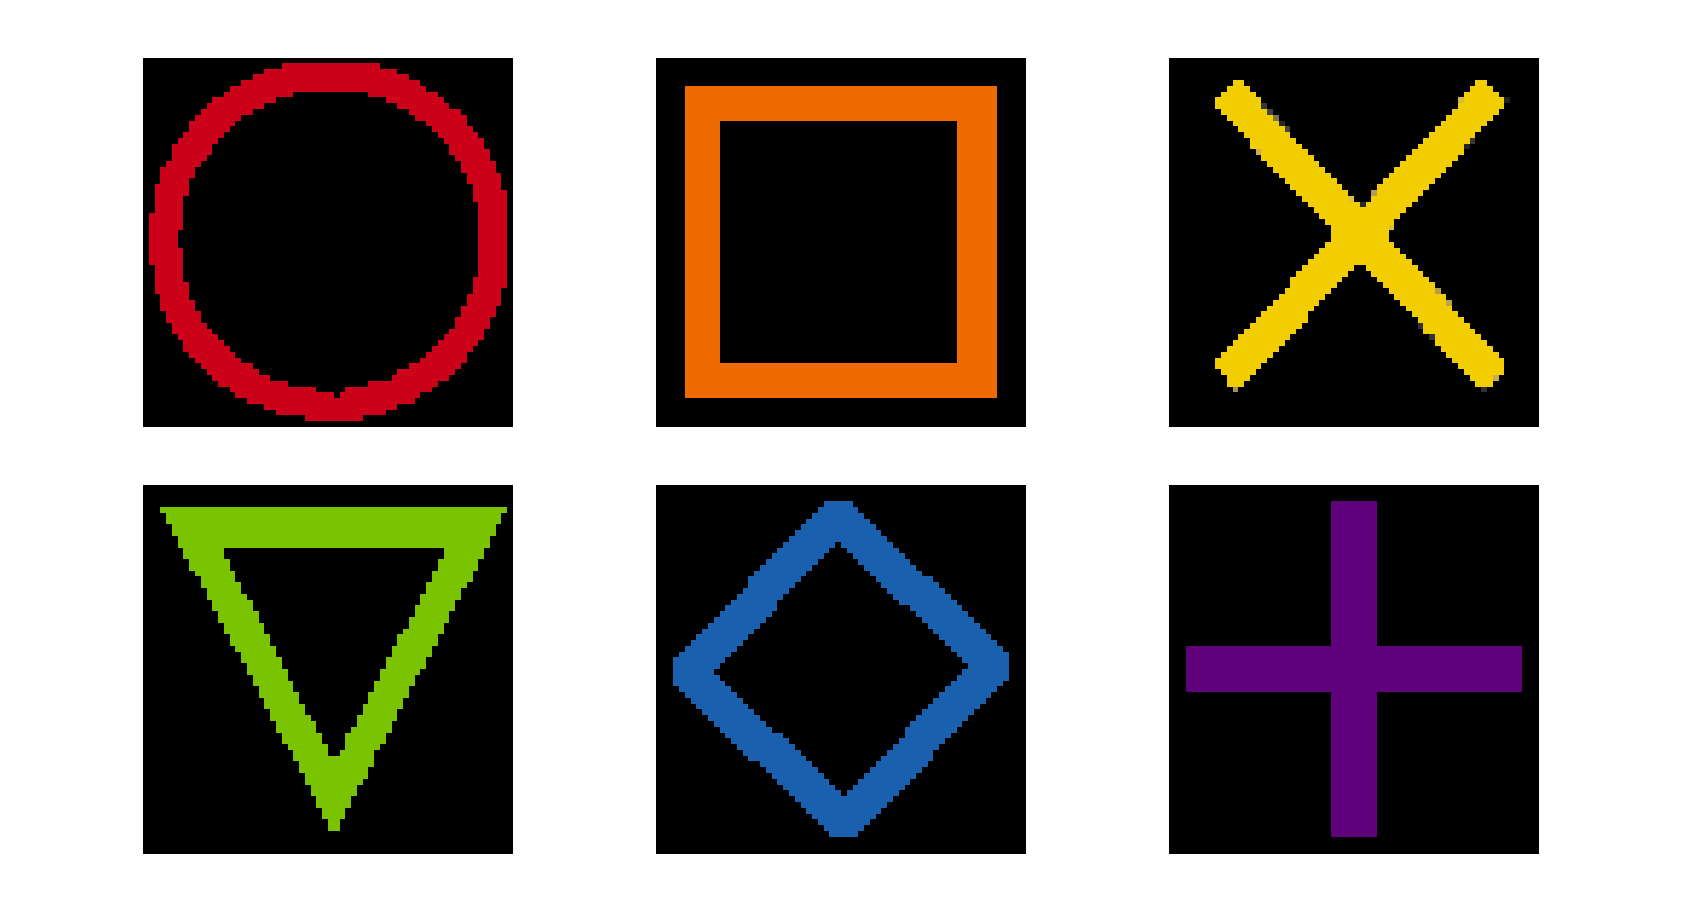
\includegraphics[width=12cm]{figuras/estimulos_cor.png}\label{fig_estimulos}
\fonte{Elaborado pelo autor (2023).}}}
\end{figure}

Foram simuladas três fases para a RNP:\@

\begin{enumerate}
  \item Simulação da rede em seu estado inicial por 1800 segundos, com um tempo médio de aparição do estímulo de 2 segundos, e
  tempo médio entre estímulos de 1 segundo. O peso das sinapses entre a retina e a rede é de 0.05.
  \item Simulação da rede também por 1800 segundos, mas com um tempo médio de aparição do estímulo de 0.2 segundo, e
  tempo médio entre estímulos de 5 segundos. O peso das sinapses entre a retina e a rede agora é de 0.1. A intenção aqui é
  fazer com que a rede tenha mais tempo entre um estímulo e outro para poder memorizá-los melhor.
  \item A última simulação é de 2400 segundos e é de onde são retirados os resultados a serem analisados. O tempo médio de aparição do estímulo diminui
  para 0.1, enquanto o tempo médio entre estímulos é de 10 segundos, com a intenção de ter uma janela maior de tempo entre os
  estímulos para analisar a capacidade de memorização da RNP.\@
\end{enumerate}


\section{Experimento 2: Formação de assembleias neuronais com sono}

De forma similar ao experimento 1, o segundo experimento consiste em simular a RNP apresentando os mesmos estímulos, mas dessa vez
com a simulação de sono. O objetivo desse experimento é analisar se a simulação de sono tem algum efeito na formação de
assembleias neuronais. A hipótese é de que a simulação do sono possa melhorar a retenção de memória, formando assembleias
neuronais mais concisas para todos os estímulos.

Esse experimento seguiu as mesmas três fases do experimento anterior, mas com a simulação do sono. Nesse experimento, a RNP ficava
em estado de vigília por 200s e dormia por 100s, seguindo uma proporção similar a de humanos que ficam acordados 16 horas por dia
e dormem 8~\cite{waterhouseDaily2012}.

\section{Análise dos resultados}

\subsection{Formação de assembleias neuronais}

O número médio de neurônios por assembleia neuronal na RNP base foi de 787, enquanto na RNP com sono foi de 432.67; isso se deve
principalmente ao fato de que as assembleias neuronais do círculo e do quadrado tiveram pouquíssimos neurônios, apenas 42 e 34 na
RNP com sono. Ambas as RNPs apresentaram dificuldades em manter uma assembleia neuronal única para o estímulo do círculo, havendo
bastante sobreposição com os neurônios da assembleia neuronal do quadrado; uma possível explicação para isso é a similaridade
entre os dois estímulos e também a possibilidade da RNP ter alcançado um limite de memória. A matriz de sobreposição das
assembleias neuronais está ilustrada nas Figura~\ref{fig_mat_base}, essa matriz é simétrica e cada número representa o número de
neurônios pertecentes a cada assembleia neuronal. Os elementos da diagonal principal da matriz indicam o número total de neurônios
em cada assembleia individual. Nos outros casos, o elemento representa quantos neurônios de uma assembleia também são parte de
outra assembleia.

\begin{figure}[!ht]
\caption{Matrizes contendo o número de neurônios pertecentes a cada assembleia neuronal.}
\centering{
\parbox{\linewidth}{
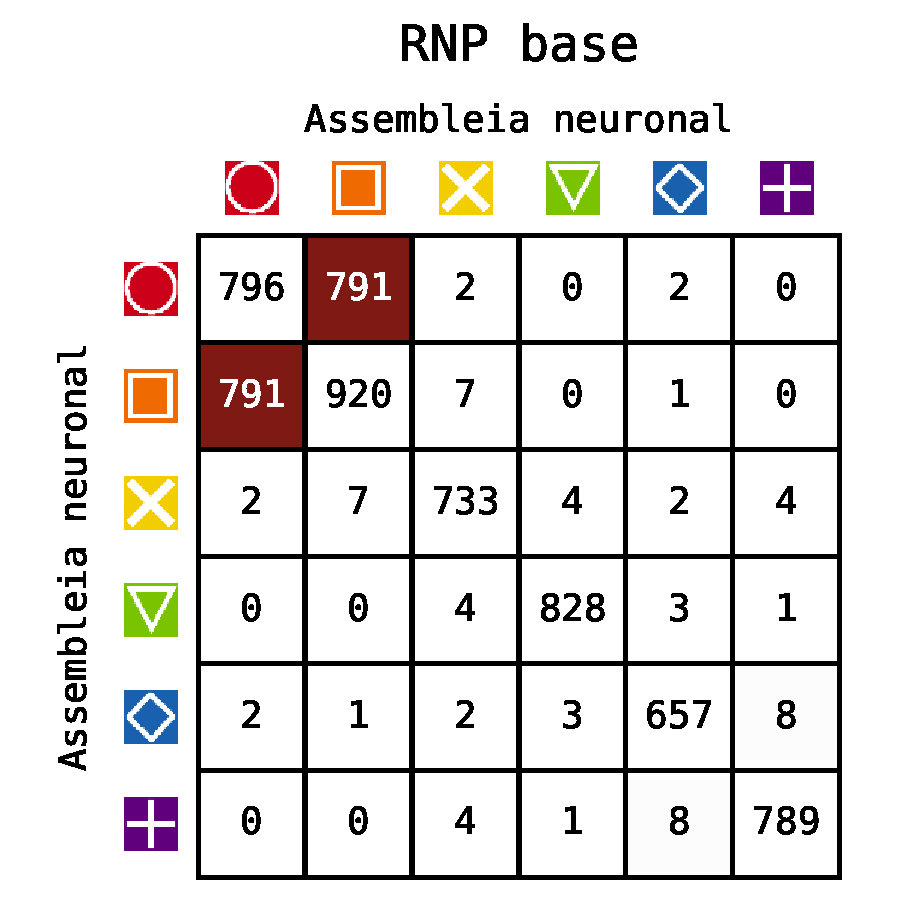
\includegraphics[width=7.5cm]{figuras/plots_pdf/RNP base.pdf}\label{fig_mat_base}
\hfill
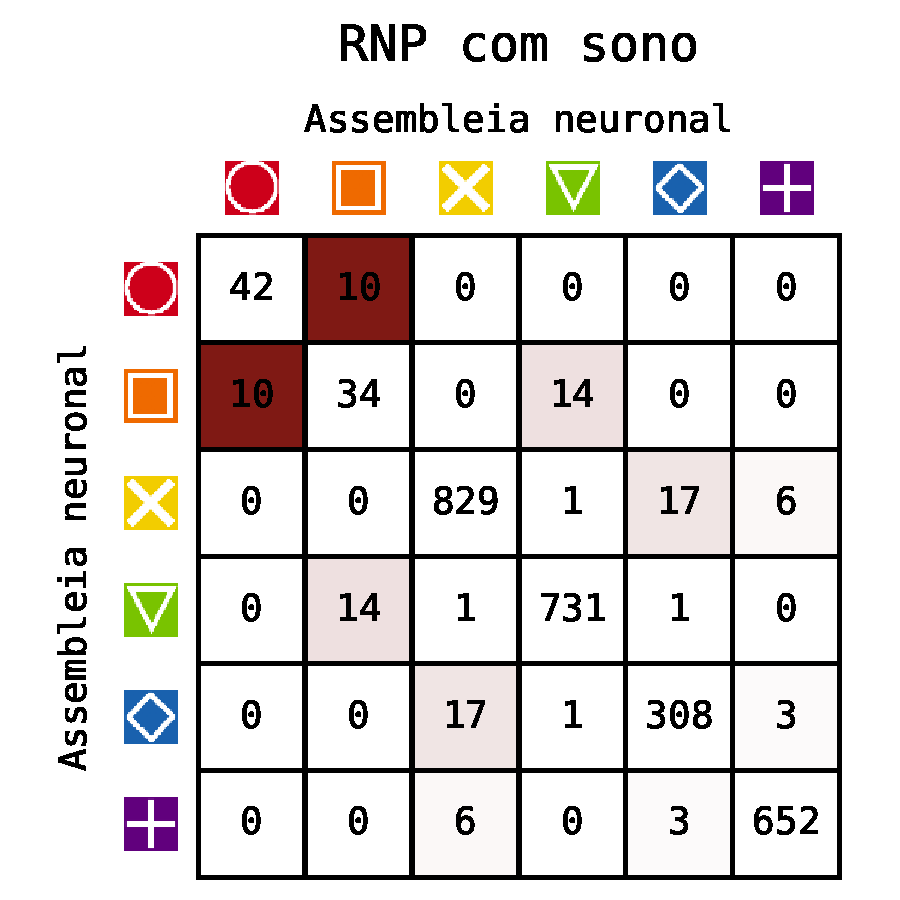
\includegraphics[width=7.5cm]{figuras/plots_pdf/RNP com sono.pdf}\label{fig_mat_sleep}
\fonte{Elaborado pelo autor (2023).}}}
\end{figure}

Outra forma de analisar o comportamento das RNPs é verificando a ativação média das assembleias neuronais para cada estímulo, como
mostra a Figura~\ref{fig_mat_act_base}. A diagonal principal claramente possui as maiores médias pois a assembleia neuronal de um
determinado estímulo apresenta atividade muito maior para esse estímulo. Nota-se também que na RNP com sono houve mais atividade
nas assembleias neuronais não relacionadas com o estímulo, indicando uma piora no desempenho.

\begin{figure}[!ht]
\caption{Matrizes representando a ativação média em Hz de cada assembleia neuronal para cada estímulo diferente.}
\centering{
\parbox{\linewidth}{
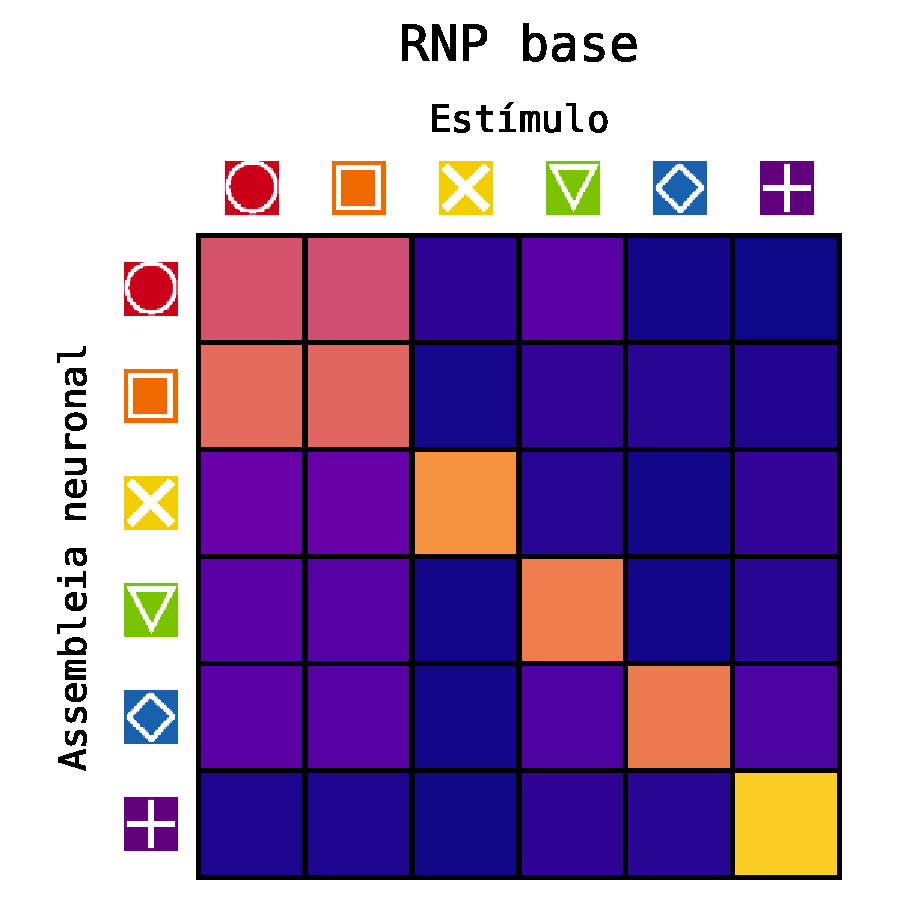
\includegraphics[height=7cm]{figuras/plots_pdf/RNP base_atv.pdf}\label{fig_mat_act_base}
\hfill
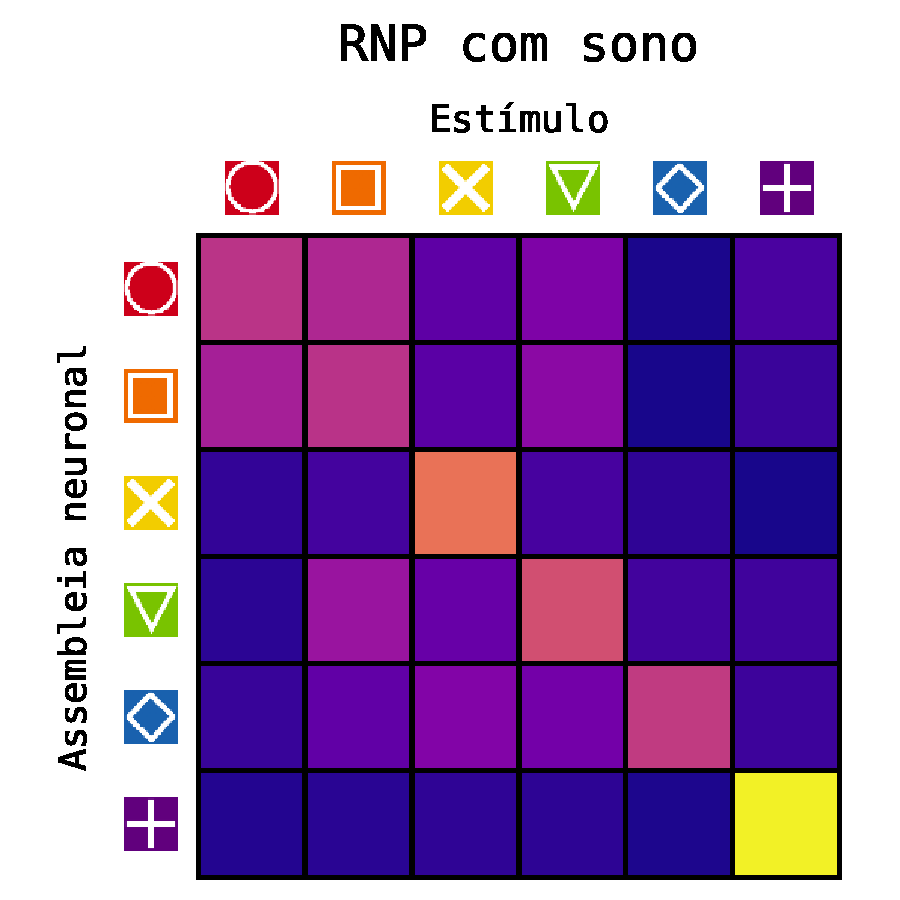
\includegraphics[height=7cm]{figuras/plots_pdf/RNP com sono_atv.pdf}\label{fig_mat_act_sono}
\hfill
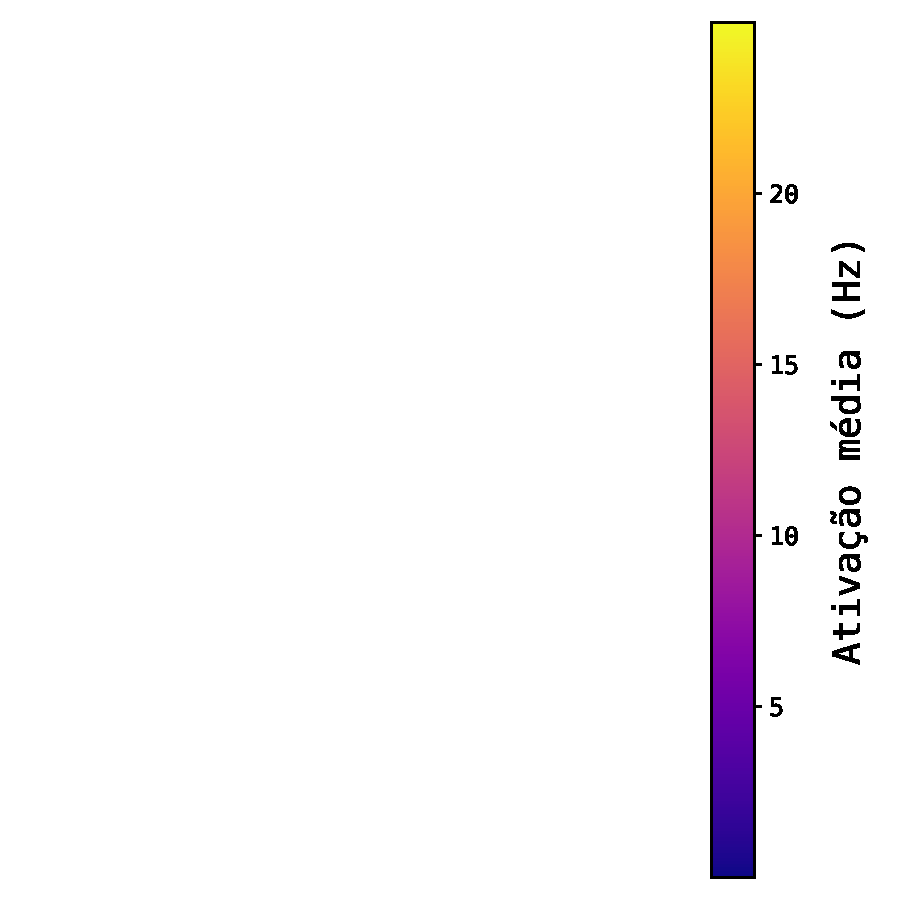
\includegraphics[height=5.8cm]{figuras/plots_pdf/atv_colorbar.pdf}\label{fig_mat_act_colorbar}
\fonte{Elaborado pelo autor (2023).}}}
\end{figure}

Os resultados deste experimento mostraram-se inconclusivos para a hipótese de que o sono poderia contribuir para a formação de
assembleias neuronais mais consistentes e, consequentemente, para a melhora no desempenho da retenção de memória.

\subsection{Atividade da RNP}

Outra forma de analisar os resultados da simulação é analisando diretamente os dados dos disparos dos neurônios. A
Figura~\ref{fig_base_act} contém um gráfico relacionando o momento dos estímulos (topo da figura) com a ativação média das
assembleias neuronais (parte inferior da figura). É possível identificar que na maioria das vezes em que um estímulo é apresentado
à RNP, a assembleia neuronal associada a esse estímulo dispara e mantém-se ativa até que outro estímulo domine a atividade da
RNP;\@ é importante notar que o estímulo é mostrado para a RNP por menos de 1 segundo, portanto a ativação da assembleia neuronal
nos segundos seguintes é a memória do estímulo.

Também pode-se notar que, quando é mostrado o estímulo do círculo ou do quadrado, as assembleias neuronais de ambos os estímulos
disparam juntas, devido à sobreposição de neurônios entre as duas assembleias neuronais discutida na seção anterior.

\begin{figure}[!ht]
\caption{Ativação das assembleias neuronais na simulação da RNP base.}
\centering{
\parbox{\linewidth}{
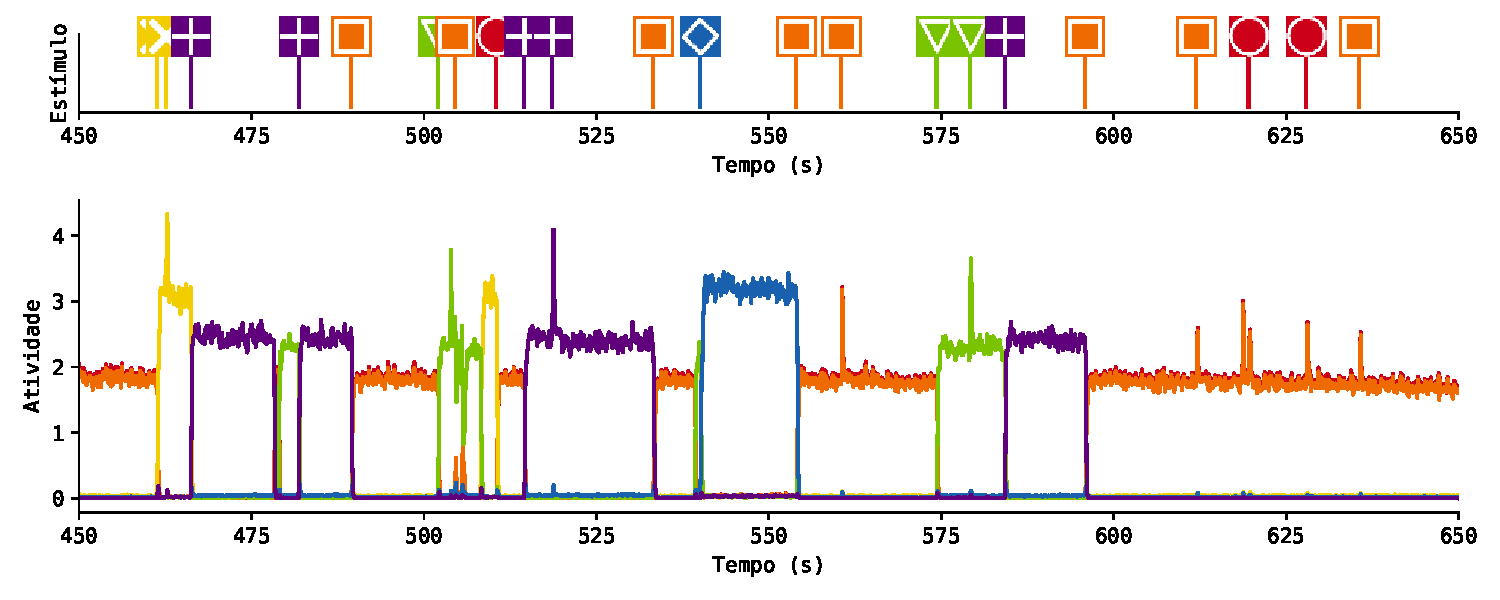
\includegraphics[width=\linewidth]{figuras/plots_pdf/atividade base.pdf}\label{fig_base_act}
\fonte{Elaborado pelo autor (2023).}}}
\end{figure}

Durante as simulações de sono da RNP, em diversas instâncias foram observados padrões intrigantes de atividade, como ilustrado nas
Figuras~\ref{fig_sleep_act} e~\ref{fig_sleep_act2}. Em várias casos, ao entrar no modo de sono, a RNP mantém uma atividade
consistente de uma assembleia neuronal, correspondente à resposta ao último estímulo mostrado a ela. Esta atividade é sustentada
por algum tempo, no entanto, há um momento em que ela diminui e é substituída por uma nova assembleia neuronal que emerge com uma
série de disparos. Como uma assembleia neuronal é a representação de uma memória na RNP, essa reativação da assembleia neuronal
sugere um momento durante o sono em que a RNP se recorda de algum estímulo.

\begin{figure}[!ht]
\caption{Ativação das assembleias neuronais na simulação da RNP com sono em momento de ``sonho''. A cor cinza indica o período de sono.}
\centering{
\parbox{\linewidth}{
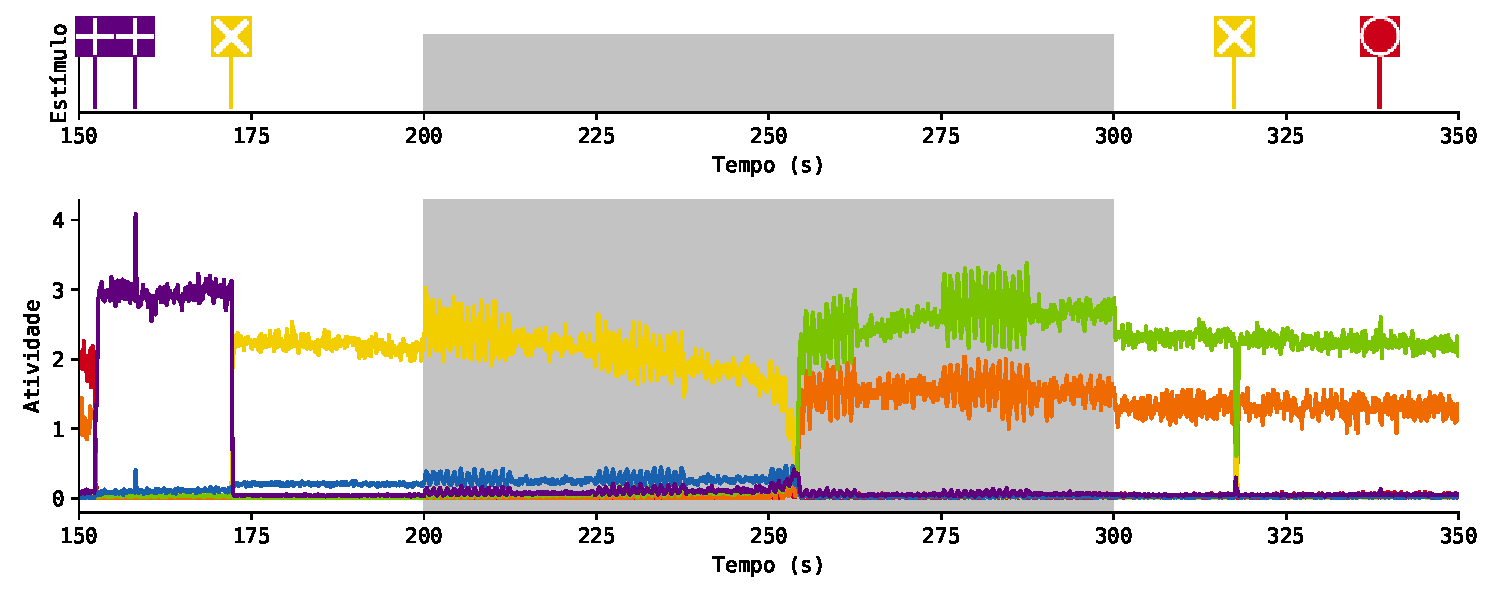
\includegraphics[width=\linewidth]{figuras/plots_pdf/atividade sonho1.pdf}\label{fig_sleep_act}
\fonte{Elaborado pelo autor (2023).}}}
\end{figure}

\begin{figure}[!ht]
\caption{Ativação das assembleias neuronais na simulação da RNP com sono em outro momento de ``sonho''. A cor cinza indica o período de sono.}
\centering{
\parbox{\linewidth}{
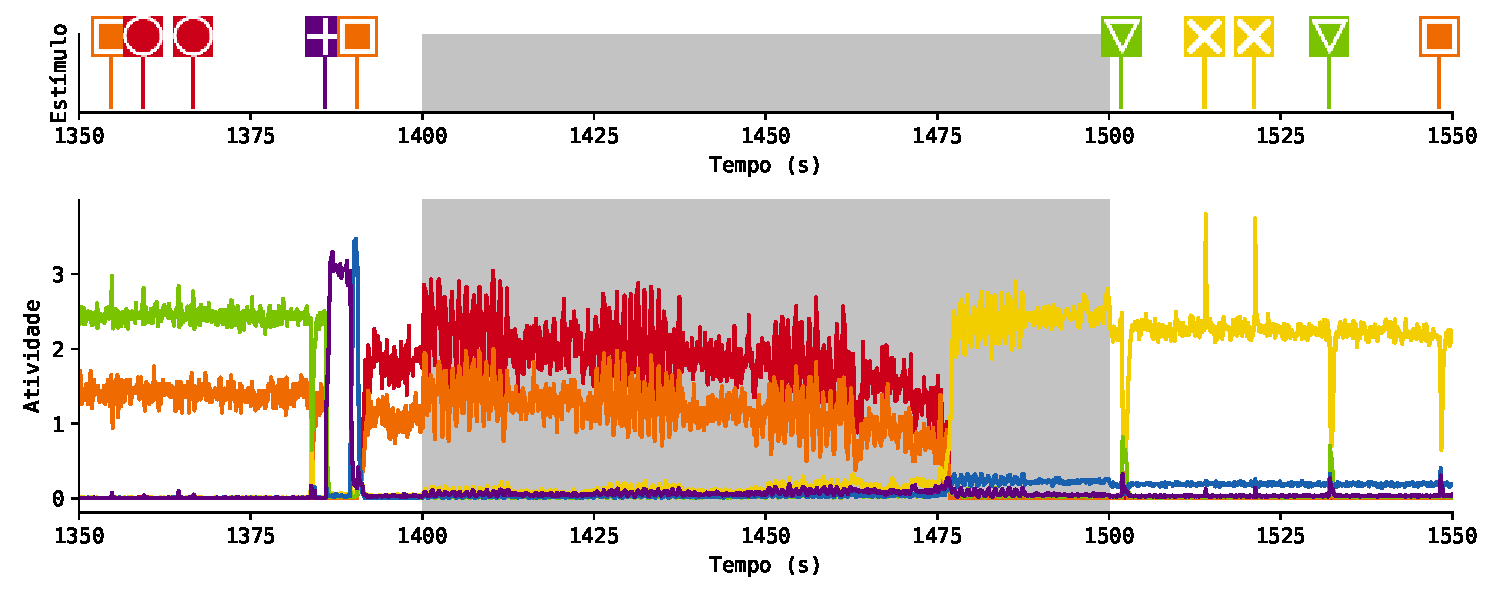
\includegraphics[width=\linewidth]{figuras/plots_pdf/atividade sonho2.pdf}\label{fig_sleep_act2}
\fonte{Elaborado pelo autor (2023).}}}
\end{figure}

Esse padrão de reativação da assembleia neuronal pode ser interpretado analogamente aos processos de sonho em organismos
biológicos. Segundo o trabalho de~\citeonline{picard-delandMemory2023}, foi observado durante o sono um fenômeno em que rastros
de memória recém-formados são reativados espontaneamente durante o sono, e esse fenômeno pode ou não estar conectado com a experiência de
sonhos e com a consolidação de memórias durante o sono.

No entanto, é fundamental abordar esta interpretação com cautela. Embora as semelhanças sejam intrigantes, é essencial
não tirar conclusões precipitadas e reconhecer que mais pesquisas são necessárias antes de afirmar que esses padrões representam
efetivamente ``sonhos'' em RNP.\@
